\documentclass[10pt]{article}
\usepackage[ngerman]{babel}
\usepackage[utf8]{inputenc}
\usepackage[T1]{fontenc}
\usepackage{graphicx}
\usepackage[export]{adjustbox}
\graphicspath{ {./images/} }
\usepackage{fvextra, csquotes}
\usepackage{amsmath}
\usepackage{amsfonts}
\usepackage{amssymb}
\usepackage[version=4]{mhchem}
\usepackage{stmaryrd}

\begin{document}
\section*{SWEN1 Summary OPENSOURCE (ohne Internet? von 11-13 nur neue Patterns, sonst nicht sep stoff)}
\begin{enumerate}
  \item März, 2024; rev. 7. Juni 2024
\end{enumerate}

Linda Riesen (rieselin)

\section*{1 Vorlesung 01}
1.1 Charakteristiken von Wasserfall, iterativ-inkrementellen und agilen Softwareentwicklungsprozessen\\
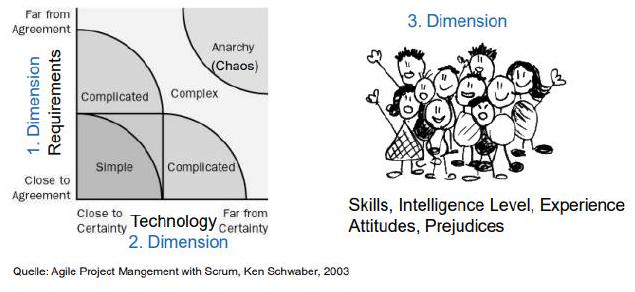
\includegraphics[max width=\textwidth, center]{2024_12_29_0d1d7b5551ea1b4b41bdg-01}

Abbildung 1: Klassifizierung Software-Entwicklungs-Probleme

\section*{Prozesse im Softwareengineering Kernprozesse}
\begin{itemize}
  \item Anforderungserhebung
  \item Systemdesign/technische Konzeption
  \item Implementierung
  \item Softwaretest
  \item Softwareeinführung
  \item Wartung/Pflege
\end{itemize}

\section*{Unterstützungsprozesse}
\begin{itemize}
  \item Projektmanagement
  \item Qualitätsmanagement
  \item Risikomanagement
\end{itemize}

Begriffe Warum wird modelliert: Um Analyse- und Designentwürfe zu diskutieren, abstimmen und zu dokumentieren bzw. zu kommunizieren. Modell: Ein Modell ist ein konkretes oder gedankliches Abbild eines vorhanden Gebildes oder Vorbild für ein zu schaffendes Gebilde (hier Softwareprodukt).\\
Original: Das Original ist das abgebildete oder zu schaffende Gebilde.\\
Modellierung: Modellierung gehört zum Fundament des Software Engineerings

\begin{itemize}
  \item Software ist vielfach (immer?) selbst ein Modell
  \item Anforderungen sind Modelle der Problemstellung
  \item Architekturen und Entwürfe sind Modelle der Lösung
  \item Testfälle sind Modelle des korrekten Funktionierens des Codes usw.\\
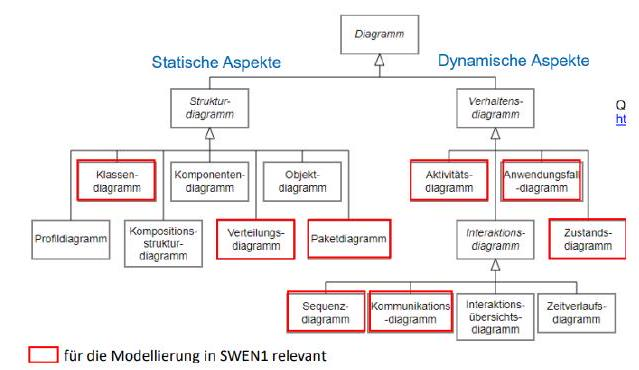
\includegraphics[max width=\textwidth, center]{2024_12_29_0d1d7b5551ea1b4b41bdg-01(1)}
\end{itemize}

Abbildung 2: Diagramme UML Übersicht

\subsection*{1.1.1 Code and Fix}
Vorgehen, bei dem Codierung oder Korrektur im Wechsel mit Ad-hoc-Tests die einzigen bewussten ausgeführten Tätigkeiten der Software-Entwicklung sind: Schnell, Agil, Einfach am Anfang, Schlecht Planbar, Schlecht Wartbar, Änderungen s. Aufwändig

\subsection*{1.1.2 Wasserfallmodell}
Die Software-Entwicklung wird als Folge von Aktivitäten/Phasen betrachtet, die durch Teilergebnisse (Dokumente) gekoppelt sind. Die Reihenfolge der Ak-\\
tivitäten ist fest definiert. : gut planbar, klare Aufteilung in Phasen, Schlechtes Risikomanagment, nie alle Anforderungen zu Anfang bekannt

\subsection*{1.1.3 Iterativ-inkrementelle Modelle}
Software wird in mehreren geplanten und kontrolliert durchgeführten Iterationen schrittweise (inkrementell) entwickelt: Flexibles Modell, Gutes Risikomanagement, Frühe Einsetzbarkeit, Planung upfront hat Grenzen, Kunde Involviert über ganze Entwicklung

Agile Softwareentwicklung Basiert auf interativ-inkrementellen Prozessmodell, Fokussiert auf gut dokumentierten und getesteten Code statt auf ausführlicher Dokumentation

\subsection*{1.2 Zweck und den Nutzen von Modellen in der Softwareentwicklung}
\begin{itemize}
  \item Modell von Requirements (close to/ far from Agreement) \& Technology (known / unknown)\\
Ein Modell ist ein konkretes oder gedankliches Abbild eines vorhanden Gebildes oder Vorbild für ein zu schaffendes Gebilde (hier Softwareprodukt).
\end{itemize}

\subsection*{1.2.1 Unified Modelling Language (UML)}
UML ist die Standardsprache für die graphische Modellierung von Anforderungen, Analyse und Entwürfen im Software Engineering (objektorientierte Modellierung). (As a sketch, blueprint, programminglanguage)

\subsection*{1.3 Artefakte in einem iterativinkrementellen Prozess illustrieren und einzuordnen}
\begin{center}
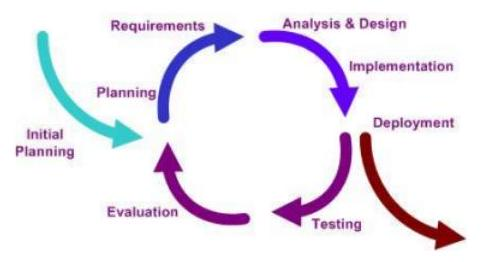
\includegraphics[max width=\textwidth]{2024_12_29_0d1d7b5551ea1b4b41bdg-02(1)}
\end{center}

Abbildung 3: Incremental Model

\section*{2 Vorlesung 02}
\section*{2.1 wichtigste Begriffe des Usability-Engineering}
\begin{center}
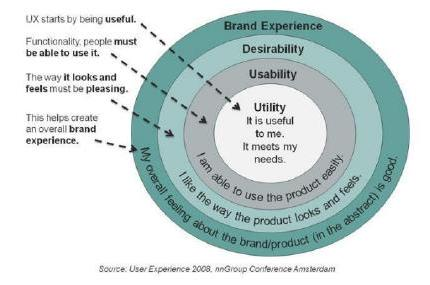
\includegraphics[max width=\textwidth]{2024_12_29_0d1d7b5551ea1b4b41bdg-02}
\end{center}

\begin{displayquote}
Abbildung 4: Usability und User Experience (UX)
\end{displayquote}

Usability = Deutsch: Gebrauchstauglichkeit\\
User Experience = Usability + Desirability\\
Customer Experience $=$ Usability + Desirability + Brand Experience

\subsection*{2.2 Usability-Anforderungen}
Die Effektivität, Effizienz und Zufriedenheit mit der die adressierten Benutzer ihre Ziele erreichen in ihren spezifischen Kontexten.

\section*{Wichtigste Aspekte}
\begin{itemize}
  \item Benutzer
  \item Seine Ziele/Aufgaben
  \item Sein Kontext
  \item Softwaresystem (inkl. UI)
\end{itemize}

\section*{Effektivität}
\begin{itemize}
  \item Der Benutzer kann alle seine Aufgaben vollständig erfüllen
  \item Mit der gewünschten Genauigkeit
\end{itemize}

Effizienz Der Benutzer kann seine Aufgaben mit minimalem/angemessenem Aufwand erledigen

\begin{itemize}
  \item Mental
  \item Physisch
  \item Zeit
\end{itemize}

\section*{Zufriedenheit Mit dem System / der Interaktion}
\begin{itemize}
  \item Minimum: Benutzer ist nicht verärgert
  \item Normal: Benutzer ist zufrieden
  \item Optimal: Benutzer ist erfreut
\end{itemize}

\subsection*{2.2.1 7 wichtige Anforderungsbereiche bezüglich Usability}
\begin{itemize}
  \item Aufgabenangemessenheit
  \item Lernförderlichkeit
  \item Individualisierbarkeit
  \item Erwartungskonformität
  \item Selbstbeschreibungsfähigkeit
  \item Steuerbarkeit
  \item Fehlertoleranz
\end{itemize}

\subsection*{2.3 User-Centered Designs}
\begin{center}
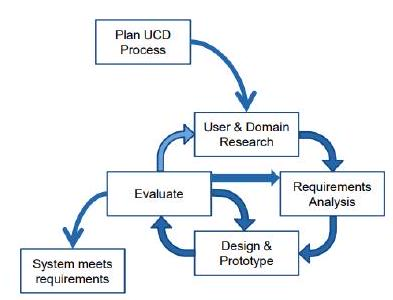
\includegraphics[max width=\textwidth]{2024_12_29_0d1d7b5551ea1b4b41bdg-03}
\end{center}

Abbildung 5: Usercentered Design

\subsection*{2.4 Ziele, Methoden und Artefakte der einzelnen Phasen des UCD}
\begin{itemize}
  \item Personas (Fiktive Person mit Eigenschaften / Fähigkeiten): Repräsentitert eine bestimmte Benutzergruppe
  \item Usage-Szenarien
  \item Mentales Modell
  \item Domänenmodell
  \item Service Blueprint / Geschäftsprozessmodell: Skizze wie Funktioniert was im Geschäft und was für Interaktionen geschehen wo
  \item Stakeholder Map\\
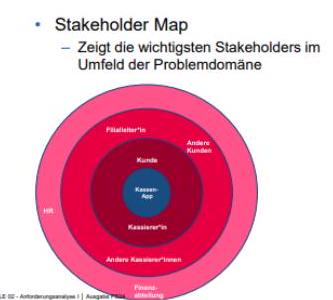
\includegraphics[max width=\textwidth, center]{2024_12_29_0d1d7b5551ea1b4b41bdg-04}
\end{itemize}

Abbildung 6: Stakeholdermap Example

\begin{itemize}
  \item Zusätzlich: UI-Skizzen der wichtigsten Screens, Wireframes (UIPrototypes), UI-Design, weitere Usability - Anforderungen
\end{itemize}

\section*{3 Vorlesung 03}
\begin{center}
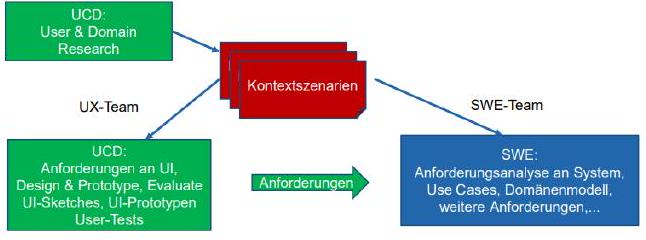
\includegraphics[max width=\textwidth]{2024_12_29_0d1d7b5551ea1b4b41bdg-04(1)}
\end{center}

Abbildung 7: Anforderungsanalyse Übersicht

\subsection*{3.1 Anforderungen aus Artefakten des UCD}
Anforderungen (Requirements): Forderungen bezüglich (Leistungs-) Fähigkeiten oder Eigenschaften die das System unter gegebenen Bedingungen erfüllen muss (explizit oder implizit)

\begin{itemize}
  \item Meist sind nie alle Anforderungen im Voraus vollständig bekannt, entwickeln sich im Laufe des Projekts
  \item Müssen mit den Benutzern und Stakeholdern erarbeitet werden
\end{itemize}

\subsection*{3.2 Anforderungen in Form von Use Cases}
Textuelle Beschreibung einer konkreten Interaktion eines Benutzers mit zukünfigem System (Beschreiben aus Sicht des Akteurs, Impkizite und Explizite Anforderungen, Ziel des Akteurs, Kontext)

\section*{3 Arten von Akteuren}
\begin{itemize}
  \item Primärakteur (Primary Actor)
  \item Initiert einen Anwendungsfall, um sein (Teil-)Ziel zu erreichen\\
Erhălt den Hauptnutzen des Anwendungsfalls\\
Beispiel Kasse: Kassier
  \item Unterstützender Akteur (Supporting Actor)
\end{itemize}

Hilft dem SuD bei der Bearbeitung eines Anwendungsfalls\\
Beispiel Kasse: externer Dienstleister wie Zahlungsdienst für Kreditkarten

\begin{itemize}
  \item Offstage-Akteur (Offstage Actor)
  \item Weitere Stakeholder, die nicht direkt mit dem System interagierten\\
Beispiel Kasse: Steuerbehörde
\end{itemize}

Abbildung 8: Arten von Akteuren

\begin{itemize}
  \item Aus Sicht des Akteurs
  \item Aktiv formuliert (Titel auch aktiv)
  \item Konkreter Nutzen
  \item Mehr als eine einzelne Interaktion / UseCase
  \item im Essentiellen, nicht Konkreten Stil (Logik, nicht Umsetzung)\\
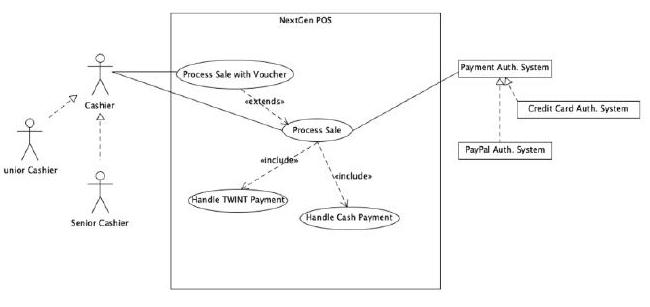
\includegraphics[max width=\textwidth, center]{2024_12_29_0d1d7b5551ea1b4b41bdg-05}
\end{itemize}

Abbildung 9: Use Case Diagramm

\subsection*{3.2.1 Brief UC}
Kurze Beschreibung des Anwendungsfalls in einem Paragraphen

\begin{itemize}
  \item Nur Erfolgsszenario
  \item Sollte enthalten:
  \item Trigger des UCs
  \item Akteure
  \item Summarischen Ablauf des UCs
  \item Wann?: Zu Beginn der Analyse
\end{itemize}

\subsection*{3.2.2 Casual UC}
Informelle Beschreibung des Anwendungsfalls in mehreren Paragraphen

\begin{itemize}
  \item Erfolgsszenario plus wichtigste Alternativszenarien
  \item Sollte enthalten:
  \item Trigger des UCs
  \item Akteure
  \item Interaktion des Akteurs mit System
  \item Wann?: Zu Beginn der Analyse
\end{itemize}

\section*{Formaler Aufbau}
\begin{itemize}
  \item UC-Name
  \item Umfang (Scope)
  \item Ebene (Level)
  \item Primärakteur (Primary Actor)
  \item Stakeholders und Interessen
  \item Vorbedingungen (Preconditions)
  \item Erfolgsgarantie/Nachbedingungen (Success
  \item Erfolgsgarantie/Nachbedingungen (Succe
\end{itemize}

Guarantee)

\begin{itemize}
  \item Standardablauf (Main Sucess Scenario)
  \item Erweiterungen (Extensions)
  \item Spezielle Anforderungen (Special Requirements)
  \item Liste der Technik und Datavariationen\\
(Technology and Data Variations)
  \item Häufigkeit des Auftretens (Frequency of Occurance
  \item Verschiedenes (Miscellaneous)
\end{itemize}

Abbildung 10: Aufbau Fully- Dressed Use Case (UC)

\subsection*{3.2.3 Systemsequenzdiagramm SSD}
Ist formal ein UML Sequenzdiagramm: Zeigt Interaktionen der Akteure mit dem System

\begin{itemize}
  \item Welche Input-Events auf das System einwirken
  \item Welche Output-Events das System erzeugt
\end{itemize}

Ziel:\\
Wichtigste Systemoperationen identifizieren, die das System zur Verfügung stellen muss (API) für einen gegebenen Anwendungsfall

\begin{itemize}
  \item Formal wie Methodenaufruf, evtl mit Parametern, Details zu Parametern sollen im Glossar erklärt werden
  \item Durchgezogener Pfel für Methodenaufruf
  \item Rückgabewert kann fehlen falls unwichtig, indirektes Update des UI, deshalb gestrichelte Linie
\end{itemize}

SSD können auch Interaktionen zwischen SuD und externen unterstützenden System zeigen\\
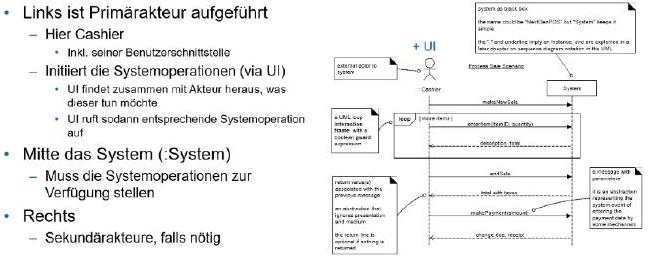
\includegraphics[max width=\textwidth, center]{2024_12_29_0d1d7b5551ea1b4b41bdg-06}

Abbildung 11: Systemsequenzdiagramm (SSD)

\section*{4 Vorlesung 04}
\subsection*{4.1 UML Klassendiagramm = Domänenmodell (vereinfachtes UML Klassendiagramm)}
Konzepte werden als Klassen modelliert, Eigenschaften als Attribute (ohne Typangabe), Assoziationen mit Multiplizitäten als Beziehung zw. Konzepten (wenn notwendig noch Aggregation (Beschriftung d Pfeile))

\subsection*{4.1.1 Konzepte: Substantive}
\begin{itemize}
  \item Physische Objekte
  \item Kataloge
  \item Container von Dingen
  \item Andere beteiligte Systeme
  \item Rollen von beteiligten Personen
  \item Artefakte (Pläne, Finanzen, Arbeit, Verträge)
  \item Zahlungsinstrumente
  \item Keine Softwareklassen
\end{itemize}

\subsection*{4.1.2 Attribute: sollen einfach/wichtig sein}
\begin{itemize}
  \item Transaktion
  \item Teil zum Ganzen
  \item Beschreibung/ Protokoll zum Gegenstand
  \item Verwendung
\end{itemize}

Attribute an Stelle von Assoziationen Verwenden Sie Assoziationen und nicht Attribute, um Konzepte in Beziehung zueinander zu setzen.

\subsection*{4.2 Analysemuster}
\subsection*{4.2.1 Beschreibungsklassen}
Artikel, Physischer Gegenstand, Diensleitung: hat Preis, Serie Nummer u Code

\subsection*{4.2.2 Generalisierung / Spezialisierung}
Wenn 100\% Regel: alle instanzen eines spezialisierten Konzepts sind auch Instanzen des generalisierten Konzepts und ÏS A"\\
Assoziationen und Attribute dienen umgekehrt als Begründung für eine gemeinsame generalisierte Klasse.

\subsection*{4.2.3 Komposition}
\subsection*{4.2.4 Zustände}
Sollen durch eigene Hierarchie dargestellt werden\\
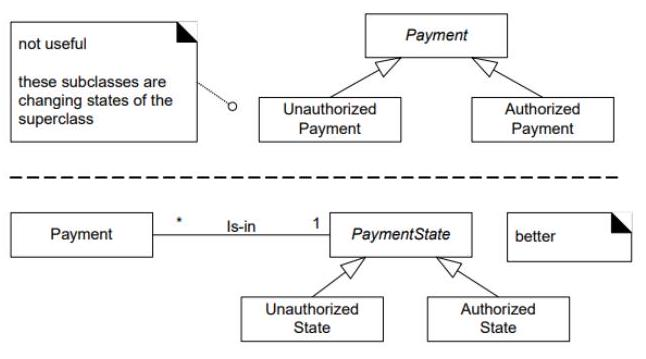
\includegraphics[max width=\textwidth, center]{2024_12_29_0d1d7b5551ea1b4b41bdg-07(1)}

Abbildung 12: Zustände Domänenmodell(DM) Beispiel

\subsection*{4.2.5 Rollen (Manager etc.)}
Dasselbe Konzept (aber selten dieselbe Instanz) kann unterschiedliche Rollen einnehmen.\\
Dargestellt als Konzepte / Assoziationen

\subsection*{4.2.6 Assoziationsklasse}
\begin{center}
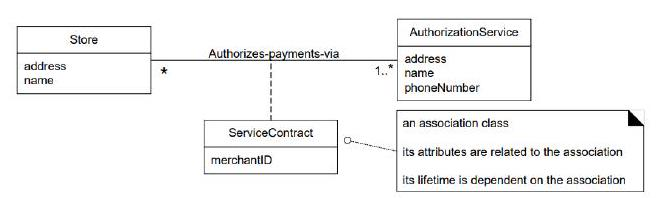
\includegraphics[max width=\textwidth]{2024_12_29_0d1d7b5551ea1b4b41bdg-07}
\end{center}

Abbildung 13: Assoziationsklasse Beispiel

\subsection*{4.2.7 Masseinheiten / Zeitintervalle}
Oft Sinnvollerweise als Konzept modelliert

\section*{5 Vorlesung 05}
\subsection*{5.1 Ubersicht Business Analyse vs Architektur vs Entwicklung}
\begin{center}
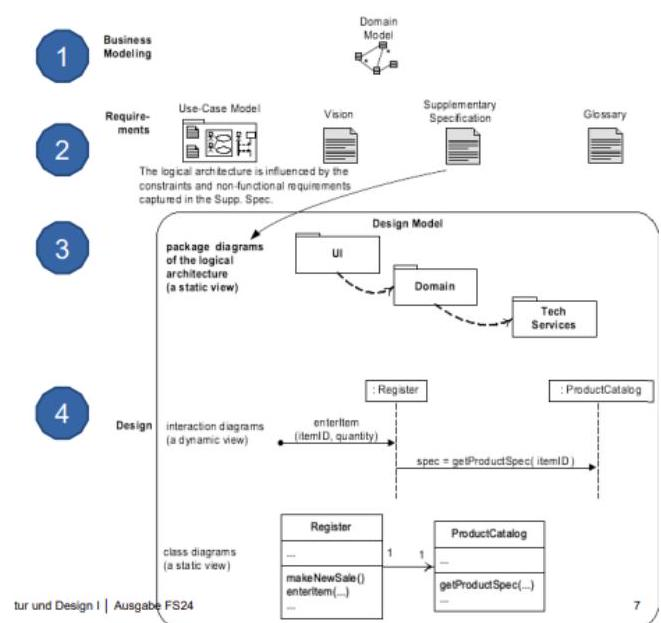
\includegraphics[max width=\textwidth]{2024_12_29_0d1d7b5551ea1b4b41bdg-07(2)}
\end{center}

Abbildung 14: Übersicht Business Analyse vs Architektur vs Entwicklung

\begin{enumerate}
  \item Domänenmodell (Business Modelling) Kontext Diagramm (Business Analyst)
  \item Requirement (Business Analyst)
  \item Logische Architektur (Software Architekt)
  \item Umsetzung (Entwicklung)\\
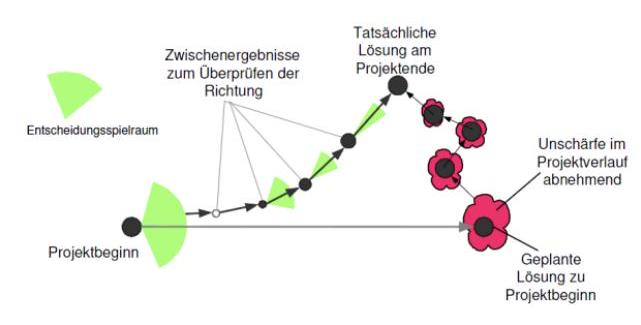
\includegraphics[max width=\textwidth, center]{2024_12_29_0d1d7b5551ea1b4b41bdg-08(1)}
\end{enumerate}

Abbildung 15: Entstehung Archtektur

\subsection*{5.2 Architektur aus Anforderungen}
Die Architektur muss heutige und zukünftige Anforderungen erfüllen können und Weiterentwicklungen der Software und seiner Umgebung ermöglichen

\subsection*{5.2.1 Architekturanalyse}
Analyse der funktionalen und nichtfunktionalen Anforderungen:\\
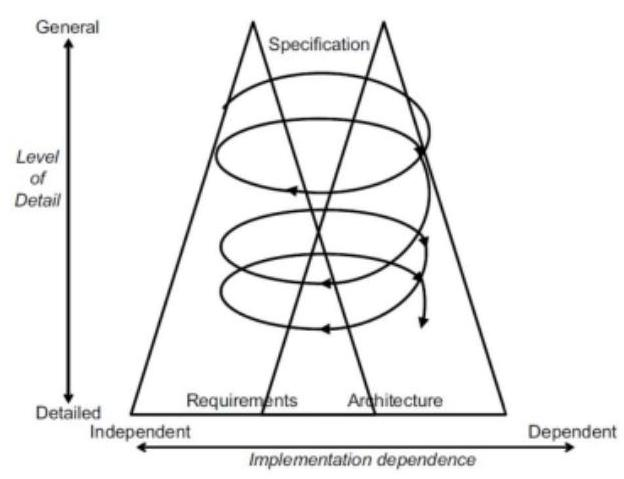
\includegraphics[max width=\textwidth, center]{2024_12_29_0d1d7b5551ea1b4b41bdg-08}

Abbildung 16: Twin Peak Model\\
Entwurfsentscheidungen sollten in erster Linie aus den Anforderungen abgeleitet werden, Architekturentscheidungen und die Konsequenzen daraus müssen mit den Stakeholdern abgestimmt werden.

\subsection*{5.2.2 ISO 25010}
\begin{itemize}
  \item ISO 25010 provides a hierarchical structure for non-functional requirements.
  \item It defines main characteristics, sub-characteristics, and metrics.
  \item Each non-functional requirement in ISO 25010 is associated with metrics.
  \item Metrics include a description of the requirement, a measurement method to check requirement fulfillment, and guidance for interpreting results.
  \item This allows for more precise and measurable formulation of requirements, which can be verified later.\\
5.2.3 Difference from FURPS + (Functionality, Usiability, Reliability, Performance, Supportability (Anpassungsfähigkeit, Wartbarkeit, etc), $+=$ Implementation, Interface, Operations, Packaging, Legal)
  \item FURPS+ is an acronym and not a standard.
  \item FURPS+ includes Functionality, Usability, Reliability, Performance, Supportability, and other terms.
\end{itemize}

\subsection*{5.2.4 Grundprinzip: Modulkonzept}
Modul (Baustein, Komponente): Güte wird gemessen mit Kohäsion und Kopplung

\begin{itemize}
  \item Möglichst autarkes Teilsystem (wenig Kopplung nach aussen)
  \item Hat eine klare minimale Schnittstelle gegen aussen
  \item Software-Modul enthält alle Funktionen und Datenstrukturen, die es benötigt
  \item Modul kann sein: Paket, Programmierkonstrukt, Library, Komponente, Service
\end{itemize}

\subsection*{5.2.5 Architektur beschreiben}
Architektur umfasst verschiedene Aspekte, die je nach Sichtweise wichtig sind

\section*{N+1 View Model + 1 View: Use Cases}
\begin{center}
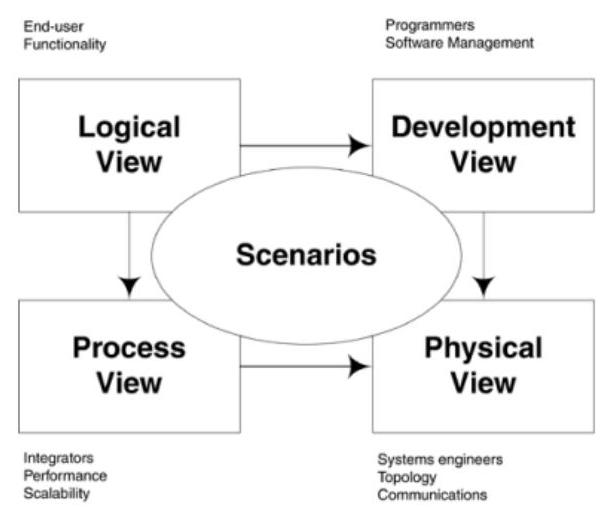
\includegraphics[max width=\textwidth]{2024_12_29_0d1d7b5551ea1b4b41bdg-09}
\end{center}

Abbildung 17: View Model\\
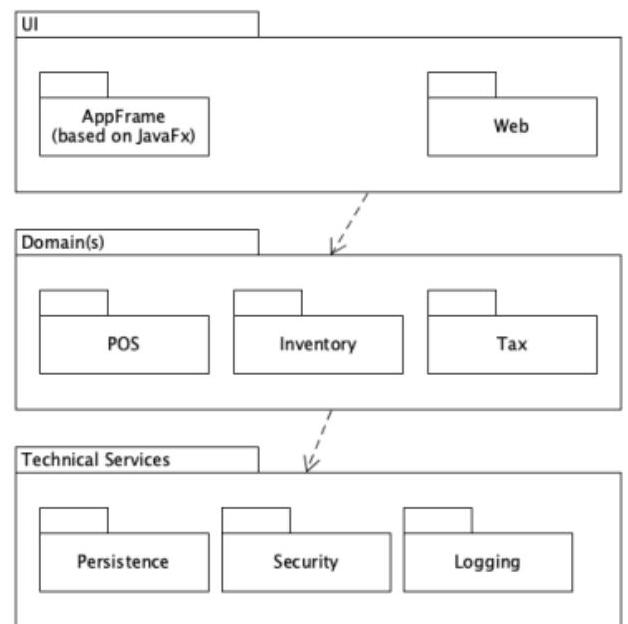
\includegraphics[max width=\textwidth, center]{2024_12_29_0d1d7b5551ea1b4b41bdg-09(1)}

Abbildung 18: UML- Paketdiagram

\begin{itemize}
  \item Mittel, um Teilsysteme zu definieren
  \item Mittel zur Gruppierung von Elementen
\end{itemize}

Paket enthält Klassen und andere Pakete

\begin{itemize}
  \item Ähnlich, aber allgemeiner als Java Packages
\end{itemize}

Abhängigkeiten zwischen Paketen\\
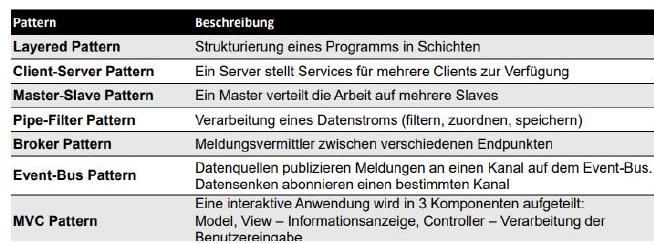
\includegraphics[max width=\textwidth, center]{2024_12_29_0d1d7b5551ea1b4b41bdg-09(2)}

Abbildung 19: Architekturpatterns

\section*{6 Vorlesung 06}
\subsection*{6.1 Zweck und Anwendung von Statischen und Dynamischen Modellen im Design}
\begin{itemize}
  \item Statische Modelle, wie beispielsweise das UML-Klassendiagramm, unterstützen den Entwurf von Paketen, Klassennamen, Attributen und Methodensignaturen (ohne Methodenkörper).
  \item Dynamische Modelle, wie beispielsweise UMLInteraktionsdiagramme, unterstützten den Entwurf der Logik, des Verhaltens des Codes und der Methodenkörper.
\end{itemize}

Statische u Dynamische ergänzen sich, werden parallel erstellt

\subsection*{6.2 Objektentwurf mit UML-Klassen-, UML-Interaktions-, UML-Zustands- und UML-Aktivitätsdiagrammen}
\subsection*{6.2.1 UML-Klassendiagramm}
Notationselemente:

\begin{itemize}
  \item Klasse, aktive Klasse
  \item Attribut
  \item Operation
  \item Sichtbarkeit von Attributen und Operationen
  \item Assoziationsname, Rollen an den Assoziationsenden
  \item Multiplizität (Bezieht sich auf die Objekte der betreffenden Klasse)
  \item Navigierbarkeit in Assoziationen
  \item Datentypen und Enumerationen
  \item Generalisierung / Spezialisierung
  \item Abstrakte Klassen
  \item Assoziation, Assoziationsklasse: Komposition, Aggregation
  \item Interface, Interface Realisierung
\end{itemize}

\subsection*{6.2.2 UML-Interkationsdiagramm}
Modellieren die Kollaborationen bzw. den Informationsaustausch zwischen Objekten (Dynamik).

Sequenzdiagramm Notationselemente:

\begin{itemize}
  \item Lebenslinie
  \item Aktionssequenz
  \item Synchrone Nachricht
  \item Antwortnachricht
  \item Gefundene, verlorene Nachricht
  \item Kombiniertes Fragment
  \item Erzeugungs-, Löschereignis
  \item Selbstaufruf
  \item Interaktionsreferenz
  \item Lebensline mit aktiver Klasse
  \item Asynchrone Nachricht
\end{itemize}

\section*{Kommuninaktionsdiagramm}
\begin{itemize}
  \item Lebenslinie (Box)
  \item Synchrone Nachricht (= Aufruf einer Operation) (Nummeriert)
  \item Antwortnachricht (= Rückgabewert)
  \item Bedingte Nachrichten «[]»
  \item Iteration «*»
\end{itemize}

\subsection*{6.2.3 UML-Zustandsdiagramm}
Welche Zustände kann ein Objekt, eine Schnittstelle, ein Use Case, ... bei welchen Ereignissen annehmen?

\begin{itemize}
  \item Start-, Endzustand
  \item einfacher Zustand
  \item Zusammengesetzter bzw. geschachtelter Zustand
  \item Flache und tiefe Historie
  \item Transition
  \item Orthogonaler Zustand
  \item Parallelisierungsknoten
  \item Synchronisationsknoten
  \item Einstiegpunkt
  \item Ausstiegspunkt
  \item Unterzustandsautomat
\end{itemize}

\subsection*{6.2.4 UML-Aktivitätsdiagramm}
Wie läuft ein bestimmter Prozess oder ein Algorithmus ab?

\begin{itemize}
  \item Aktivität
  \item Aktionsknoten (Aktion)
  \item Objektknoten (Objekt)
  \item Entscheidungs- und Vereinigungsknoten
  \item Kante
  \item Initialknoten
  \item Aktivitätsendknoten
  \item Partition (auch Swimlane genannt)
  \item Parallelisierungsknoten
  \item Synchronisationsknoten
  \item SendSignal-Aktion
  \item Ereignis- bzw. Zeitereignisannahmeaktion
  \item CallBehavior-Aktion
\end{itemize}

\subsection*{6.3 Responsibility Driven Design (RDD)}
Denken in Verantwortlichkeiten, Rollen und Kollaborationsbeziehungen für den Entwurf von Softwareklassen.\\
RDD kann auf jeder Ebene des Designs angewendet werden (Klasse, Komponente, Schicht).\\
Verantwortlichkeiten werden durch Attribute und Methoden implementiert.

\subsection*{6.4 Prinizpien für Klassenentwurf: GRASP, SOLID}
\subsection*{6.4.1 SOLID: Missing from Slides}
6.4.2 GRASP (General Responsibility Assignment Software Patterns)

\begin{itemize}
  \item welche Klassen und Objekte wofür zuständig
  \item für erleichterung Kommunikation d Entwickler
  \item grundlegenden Prinzipen bzw. Pattern
  \item Information Expert: Ein Objekt sollte die Verantwortung für eine Aufgabe übernehmen, wenn es die benötigten Informationen dazu besitzt.
  \item Creator: Ein Objekt sollte für die Erstellung von anderen Objekten verantwortlich sein, wenn eine starke Beziehung zwischen ihnen besteht.
  \item Controller: Ein Objekt sollte die zentrale Steuerungslogik in einem System repräsentieren.
  \item Low Coupling: Objekte sollten lose miteinander gekoppelt sein, um die Flexibilität und Wiederverwendbarkeit des Systems zu erhöhen.
  \item High Cohesion: Eine Klasse sollte nur zusammengehörige Funktionen und Daten enthalten, um ihre Verständlichkeit und Wartbarkeit zu verbessern.
  \item Polymorphism: Objekte sollten so entworfen werden, dass sie anhand ihrer Schnittstellen verwendet werden können, unabhängig von ihrer spezifischen Implementierung.
  \item Pure Fabrication: Künstliche Klassen sollten erstellt werden, um eine hohe Kohäsion und niedrige Kopplung zu erreichen, wenn keine natürliche Klasse die Verantwortung übernehmen kann.
  \item Indirection: Zwischen Objekten sollten indirekte Verbindungen hergestellt werden, um die Flexibilität und Wartbarkeit zu erhöhen.
  \item Protected Variations: Mechanismen sollten eingeführt werden, um Variationen in den Systemkomponenten zu schützen und unerwünschte Auswirkungen von Änderungen zu minimieren.
\end{itemize}

\section*{7 Vorlesung 07}
\subsection*{7.1 Use Cases und Use-Case-Realization}
Die Planung erfolgt anhand von Use-Cases, Realisierung v Use-Cases\\
Der wichtigste Teil sind die detaillierten Szenarien (Standardszenario und Erweiterungen), und davon die Systemantworten. Diese müssen schlussendlich realisiert werden.

\subsection*{7.1.1 Vergleich SSD}
UI statt System, Systemoperationen sind Elemente die realisiert werden

\subsection*{7.1.2 Warum UML}
\begin{itemize}
  \item Zwischenschritt bei wenig Erfahrung
  \item Ersatz für Programmiersprache, Kompakt
  \item auch für Laien zu verstehen
\end{itemize}

\subsection*{7.2 Vorgehen UC Realization}
\begin{enumerate}
  \item Use Case auswählen, offene Fragen klären, SSD ableiten
  \item Systemoperation auswählen
  \item Operation Contract (Systemvertrag) erstellen/überlegen
  \item Aktuellen Code/Dokumentation analysieren\\
(a) DCD überprüfen/aktualisieren\\
(b) Vergleich mit Domänenmodell durchführen\\
(c) Neue Klassen gemäß Domänenmodell erstellen
  \item Falls notwendig, Refactorings durchführen\\
(a) Controller Klasse bestimmen\\
(b) Zu verändernde Klassen festlegen\\
(c) Weg zu Klassen festlegen\\
i. Weg mit Parametern wählen\\
ii. Klassen ggf. neu erstellen\\
iii. Verantwortlichkeiten zuweisen\\
iv. Varianten bewerten\\
(d) Veränderungen programmieren\\
(e) Review durchführen
\end{enumerate}

\section*{8 Vorlesung 08}
\subsection*{8.1 Allgemeiner Aufbau u Zweck von Design Pattern (DP)}
\begin{itemize}
  \item bewährte Lösungen f wiederkehrende Probleme schnell finden
  \item effiziente Kommunikation
  \item immer tradeoff zw. Flexibilität u Kompatibilität
  \item Programm wird nicht besser mit DP
\end{itemize}

\subsection*{8.1.1 Adapter}
Ermöglicht die Zusammenarbeit von Objekten mit inkompatiblen Schnittstellen. (Überall wo Dienste angesprochen werden, die austauschbar sein sollten)

\subsection*{8.1.2 Simple Factory}
(eigene Klasse) erstellt Objekte, die aufwändig zu erzeugen sind

\subsection*{8.1.3 Singleton}
Stellt sicher, dass eine Klasse nur eine Instanz hat und einen globalen Zugriffspunkt darauf bereitstellt.

\subsection*{8.1.4 Dependency Injection}
Ermöglicht es, einem abhängigen Objekt die benötigten Abhängigkeiten bereitzustellen. (Ersatz f Facotry Pattern)

\subsection*{8.1.5 Proxy}
Bietet einen Platzhalter (mit demselben Interface) für ein anderes Objekt, um den Zugriff darauf zu kontrollieren. Proxy Objekt leitet alle Methodenaufrufe zum richtigen Objekt weiter

\begin{itemize}
  \item Remote Proxy: Stellvertreter für ein Objekt in einem anderen Adressraum und übernimmt die Kommunikation mit diesem.
  \item Virtual Proxy: Verzögert das Erzeugen des richtigen Objekts bis zum ersten Mal, dass es benutzt wird.
  \item Protection Proxy: Kontrolliert den Zugriff auf das richtige Objekt.
\end{itemize}

\subsection*{8.1.6 Chain of Responsibility}
Ermöglicht es einem Objekt, eine Anfrage entlang einer Kette potenzieller Handler zu senden, bis einer die Anfrage behandelt. (wenn unklar im vorraus welcher Handler zuständig sein wird)

\section*{9 Vorlesung 09}
\subsection*{9.1 Decorator}
\subsection*{9.1.1 Problem}
Ein Objekt (nicht eine ganze Klasse) soll mit zusätzlichen Verantwortlichkeiten versehen werden.

\subsection*{9.1.2 Solution}
Ein Decorator, der dieselbe Schnittstelle hat wie das ursprüngliche Objekt, wird vor dieses geschaltet. Der Decorator kann nun jeden Methodenaufruf entweder selber bearbeiten, ihn an das ursprüngliche Objekt weiterleiten oder eine Mischung aus beidem machen.

\subsection*{9.2 Observer}
\subsection*{9.2.1 Problem}
Ein Objekt soll ein anderes Objekt benachrichtigen, ohne dass es den genauen Typ des Empfängers kennt.

\subsection*{9.2.2 Solution}
Ein Interface wird definiert, das nur dazu dient, ein Objekt über eine Änderung zu informieren. Dieses Interface wird vom «Observer» implementiert. Das\\
«Observable» Objekt benachrichtigt alle registrierten «Observer» über eine Änderung.

\subsection*{9.3 Strategy}
\subsection*{9.3.1 Problem}
Ein Algorithmus soll einfach austauschbar sein.

\subsection*{9.3.2 Solution}
Den Algorithmus in eine eigene Klasse verschieben, die nur eine Methode mit diesem Algorithmus hat.\\
Ein Interface für diese Klasse definieren, das von alternativen Algorithmen implementiert werden muss

\subsection*{9.4 Composite}
\subsection*{9.4.1 Problem}
Eine Menge von Objekten haben dasselbe Interface und müssen für viele Verantwortlichkeiten als Gesamtheit betrachtet werden.

\subsection*{9.4.2 Solution}
Sie definieren ein Composite, das ebenfalls dasselbe Interface implementiert und Methoden an die darin enthaltenen Objekte weiterleitet

\subsection*{9.5 State}
\subsection*{9.5.1 Problem}
Das Verhalten eines Objekts ist abhängig von seinem inneren Zustand.

\subsection*{9.5.2 Solution}
Das Objekt hat ein darin enthaltenes Zustandsobjekt.\\
Alle Methoden, deren Verhalten vom Zustand abhängig sind, werden über das Zustandsobjekt geführt.

\subsection*{9.6 Visitor}
\subsection*{9.6.1 Problem}
Eine Klassenhierarchie soll um (weniger wichtige) Verantwortlichkeiten erweitert werden, ohne dass viele neue Methoden hinzukommen.

\subsection*{9.6.2 Solution}
Die Klassenhierarchie wird mit einer Visitor-Infrastruktur erweitert. Alle weiteren neuen Verantwortlichkeiten werden dann mit spezifischen VisitorKlassen realisiert.

\subsection*{9.7 Facade}
\subsection*{9.7.1 Problem}
Sie setzen ein ziemlich kompliziertes Subsystem mit vielen Klassen ein. Wie können Sie seine Verwendung so vereinfachen, dass alle Team-Mitglieder es korrekt und einfach verwenden können?

\subsection*{9.7.2 Solution}
Eine Facade (Fassade) Klasse wird definiert, welche eine vereinfachte Schnittstelle zum Subsystem anbietet und die meisten Anwendungen abdeckt.

\subsection*{9.8 Abstract Factory}
\subsection*{9.8.1 Problem}
Sie müssen verschiedene, aber verwandte Objekte erstellen, ohne ihre konkreten Klassen anzugeben. Wie können Sie die Erstellung der Objektfamilien zentralisieren und von ihrer konkreten Implementierung abstrahieren?

\subsection*{9.8.2 Solution}
Das Abstract Factory Muster definiert eine Schnittstelle zur Erstellung von Familien verwandter oder abhängiger Objekte, ohne ihre konkreten Klassen zu benennen. Es bietet Methoden, um Objekte der verschiedenen Produktfamilien\\
zu erstellen, und ermöglicht es, ganze Produktfamilien konsistent zu verwenden.

\subsection*{9.9 Factory Method}
\subsection*{9.9.1 Problem}
Es gibt eine Oberklasse, aber die genauen Unterklassen sollen durch eine spezielle Logik zur Laufzeit bestimmt werden. Wie können Sie die Instanziierung dieser Klassen so gestalten, dass sie flexibel und erweiterbar bleibt?

\subsection*{9.9.2 Solution}
Das Factory Method Muster definiert eine Schnittstelle zur Erstellung eines Objekts, lässt aber die Unterklassen entscheiden, welche Klasse instanziiert wird. Dadurch wird die Erstellung der Objekte auf Unterklassen delegiert, wodurch die Klasse flexibler und erweiterbar wird.

\subsection*{9.10 Command}
\subsection*{9.10.1 Problem}
Sie müssen eine Anforderung in Form eines Objekts kapseln, um parameterisierte Clients, Warteschlangen oder Log-Requests sowie Operationen rückgängig machen zu können. Wie können Sie dies strukturieren?

\subsection*{9.10.2 Solution}
Das Command Muster kapselt eine Anforderung als Objekt, wodurch Sie Parameter für Clients, Warteschlangen oder Log-Requests einfügen und Operationen rückgängig machen können. Es besteht aus einem Kommando-Objekt, das eine bestimmte Aktion mit ihren Parametern, Empfänger und eventuell einer Methode zur Rückgängigmachung enthält.

\subsection*{9.11 Template Method}
\subsection*{9.11.1 Problem}
In einer Methode einer Oberklasse gibt es einige Schritte, die in Unterklassen unterschiedlich implementiert werden sollen, während die Struktur der Methode erhalten bleiben muss. Wie können Sie die Schritte anpassbar machen?

\subsection*{9.11.2 Solution}
Das Template Method Muster definiert das Skelett eines Algorithmus in einer Methode, wobei einige Schritte von Unterklassen implementiert werden. Es ermöglicht Unterklassen, bestimmte Schritte des Algorithmus zu überschreiben, ohne die Struktur des Algorithmus zu verändern.

\section*{10 Vorlesung 10}
\subsection*{10.1 Quellcode aus Design Artefakten ableiten}
\subsection*{10.1.1 Umsetzungs-Reihenfolge: Variante Bottom-Up}
Kurze Erklärung: Implementierung beginnt mit Basisbausteinen, die schrittweise zu größeren Teilen kombiniert werden.\\
Vorgehen: Start mit Basisfunktionalitäten, dann schrittweise Erweiterung und Integration.\\
Eigenschaften: Gründlich, bietet solide Basis, gut für sich ändernde Anforderungen.

\subsection*{10.1.2 Umsetzungs-Reihenfolge: Variante Agile}
Kurze Erklärung: Flexible, inkrementelle Entwicklung in kurzen Iterationen. Vorgehen: Kontinuierliche Lieferung funktionsfähiger Teile in Sprints, Anpassung an sich ändernde Anforderungen.\\
Eigenschaften: Hohe Flexibilität, schnelles Feedback, geeignet für sich ändernde Anforderungen.

\subsection*{10.2 Codier-Richtlinien}
\section*{Abmachung für:}
\begin{itemize}
  \item Fehlerbehandlung
  \item Codierrichtlinien (Gross/Kleinschreibung, Einrücken, Klammernsetzung, Prüf programme)
  \item Namensgebung f. Klasse, Attribute, Methoden, Variablen
\end{itemize}

\subsection*{10.3 Implementierungs- / Umsetzungsstrategie}
\section*{Code-Driven Development}
\begin{itemize}
  \item Zuerst die Klasse implementieren
\end{itemize}

\section*{TDD: Test-Driven Development}
\begin{itemize}
  \item Zuerst Tests für Klassen/Komponenten schreiben, dann den Code entwickeln
\end{itemize}

\section*{BDD: Behavior-Driven Development}
\begin{itemize}
  \item Tests aus Benutzersicht beschreiben
  \item Zum Beispiel durch die Business Analysten mit Hilfe von Gherkin
\end{itemize}

\subsection*{10.4 Laufzeit Optimierung, Optimierungsregeln}
\begin{itemize}
  \item Optimiere nicht sofort, sondern analysiere zuerst, wo Zeit tatsächlich verbraucht wird.
  \item Verwende Performance-Monitoring-Tools, um Zeitfresser zu identifizieren.
  \item Besonders kritisch sind Datenbankzugriffe pro Objekt über eine Liste.
  \item Überprüfe und optimiere Algorithmen, z.B. Collections.sort() in Java 7.
  \item Bedenke, dass moderne Compiler bereits viel Optimierung leisten.
  \item Ziehe Berechnungen aus Schleifen heraus, da die Java VM und Just-In-Time-Compilation diese optimieren.
\end{itemize}

\subsection*{10.5 Refactoring}
Definition: Strukturierte Methode zum Umstrukturieren vorhandenen Codes, ohne das externe Verhalten zu ändern. Ziele:

\begin{itemize}
  \item Verbesserung der internen Struktur durch viele kleine Schritte.
  \item Trennung vom eigentlichen Entwicklungsprozess.
  \item Verbesserung des Low-Level-Designs und der Programmierpraktiken.
\end{itemize}

\section*{Methoden zur Code-Verbesserung:}
\begin{itemize}
  \item DRY: Vermeidung von dupliziertem Code.
  \item Klare Namensgebung für erhöhte Lesbarkeit.
  \item Aufteilung langer Methoden in kleinere, klar definierte Teile.
  \item Strukturierung von Algorithmen in Initialisierung, Berechnung und Ergebnisverarbeitung.
  \item Verbesserung der Sichtbarkeit und Testbarkeit.
\end{itemize}

Code Smells:

\begin{itemize}
  \item Duplizierter Code
  \item Lange Methoden
  \item Klassen mit vielen Instanzvariablen oder viel Code
  \item Auffällig ähnliche Unterklassen
  \item Fehlen von Interfaces oder hohe Kopplung zwischen Klassen
\end{itemize}

\section*{Unterstützung durch:}
\begin{itemize}
  \item Automatisierte Tests zur Sicherstellung der Funktionsfähigkeit nach Refactoring.
  \item Moderne Entwicklungsumgebungen, die abhängige Arbeitsschritte automatisieren.
\end{itemize}

\section*{Refactoring Patterns:}
\begin{itemize}
  \item Umbenennung von Methoden, Klassen und Variablen für klarere Bezeichnungen.
  \item Verschieben von Methoden in Super- oder Subklassen.
  \item Extrahieren von Teilfunktionen in separate Methoden oder Konstanten.
  \item Einführung erklärender Variablen zur Verbesserung der Lesbarkeit.
\end{itemize}

\subsection*{10.6 Testing}
\subsection*{10.6.1 Grundlegende Testarten}
\begin{itemize}
  \item Funktionaler Test (Black-Box Verfahren): Überprüft die Funktionalität des Systems, ohne den internen Code zu kennen.
  \item Nicht funktionaler Test (Lasttest etc.): Testet nicht-funktionale Anforderungen wie Leistung, Skalierbarkeit, usw.
  \item Strukturbezogener Test (White-Box Verfahren): Überprüft die interne Struktur des Codes, um sicherzustellen, dass alle Pfade abgedeckt sind.
  \item Änderungsbezogener Test (Regressionstest etc.): Überprüft, ob durch Änderungen im Code keine neuen Fehler eingeführt wurden.
  \item Integrationstest
  \item Systemtest
  \item Abnahmetest
  \item Regressionstest
\end{itemize}

\subsection*{10.6.2 Wichtige Begriffe}
\begin{itemize}
  \item Testling, Testobjekt: Objekt, das getestet wird
  \item Fehler: Fehler, den der Entwickler macht
  \item Fehlerwirkung, Bug: Jedes Verhalten, das von den Spezifikationen abweicht
  \item Testfall: Satz von Testdaten zur vollständigen Ausführung eines Tests
  \item Testtreiber: Programm, das den Test startet und ausführt
\end{itemize}

\subsection*{10.6.3 Merkmale}
Was wird getestet?

\begin{itemize}
  \item Einheit / Klasse (Unit-Test)
  \item Zusammenarbeit mehrerer Klassen
  \item Gesamte Applikationslogik (ohne UI)
  \item Gesamte Anwendung (über UI)
\end{itemize}

Wie wird getestet?

\begin{itemize}
  \item Dynamisch: Testfall wird ausgeführt (Black-Box / White-Box Test)
  \item Statisch: Quelltext wird analysiert (Walkthrough, Review, Inspektion)
\end{itemize}

\section*{Wann wird der Test geschrieben?}
\begin{itemize}
  \item Vor dem Implementieren (Test-Driven Development, TDD)
  \item Nach dem Implementieren
\end{itemize}

\section*{Wer testet?}
\begin{itemize}
  \item Entwickler
  \item Tester, Qualitätssicherungsabteilung
  \item Kunde, Endbenutzer
\end{itemize}

\section*{11 Vorlesung 11}
\subsection*{11.1 Verteiltes System Definition + Einsatz}
Ein verteiltes System besteht aus einer Sammlung autonomer Computer (Knoten) und Softwarebausteinen (Komponenten), die über ein Netzwerk miteinander verbunden sind und gemeinsam als ein einziges System arbeiten. Sie werden in verschiedenen Bereichen eingesetzt, darunter Datenbanken, CloudComputing, verteilte Anwendungen usw.

\begin{itemize}
  \item Oft sehr gross
  \item Sehr datenorientiert: Datenbanken im Zentrum der Anwendung
  \item Extrem interaktiv: GUI, aber auch Batch
  \item Sehr nebenläufig: Grosse Anzahl an parallel arbeitenden Benutzern
  \item Oft hohe Konsistenzanforderungen
\end{itemize}

\subsection*{11.2 Verteiltes System Konzepte + Architekturstil}
Verteilte Systeme basieren auf verschiedenen Konzepten und Architekturstilen:

\subsection*{11.2.1 Kommunikationsverfahren}
Kommunikationsverfahren umfassen Methoden, mit denen die einzelnen Knoten in einem verteilten System miteinander kommunizieren können. Dazu gehören beispielsweise Remote Procedure Calls (RPC), Message Queuing und Publish-Subscribe-Systeme.

\subsection*{11.2.2 Fehlertoleranz}
Fehlertoleranz ist ein wichtiger Aspekt verteilter Systeme, der sicherstellt, dass das System auch bei Ausfällen oder Fehlern in einzelnen Komponenten weiterhin zuverlässig arbeitet. Hierzu werden Mechanismen wie Replikation, Failover und Fehlererkennung eingesetzt.

\subsection*{11.2.3 Fehlersemantik}
Die Fehlersemantik beschreibt das Verhalten eines verteilten Systems im Falle von Fehlern oder Ausfällen. Dies umfasst Aspekte wie Konsistenzgarantien, Recovery-Verfahren und Kompensationsmechanismen.

\subsection*{11.3 Design- und Implementierungsaspekte von Client-ServerSystemen}
Client-Server-Systeme sind eine häufige Architektur für verteilte Systeme, bei der Clients Anfragen an einen zentralen Server senden, der diese verarbeitet und entsprechende Antworten zurückgibt. Design- und Implementierungsaspekte umfassen unter anderem die Aufteilung von Funktionalitäten zwischen Client und Server, die Wahl der Kommunikationsprotokolle und die Skalierbarkeit des Systems.

\subsection*{11.4 Verteiltes System Architektur + Design Patterns}
Die Architektur verteilter Systeme kann durch verschiedene Design Patterns strukturiert werden, um wiederkehrende Probleme effizient zu lösen. Dazu gehören Patterns wie Master-Slave, Peer-to-Peer, Publish-Subscribe, sowie verschiedene Replikations- und Verteilungsstrategien.\\
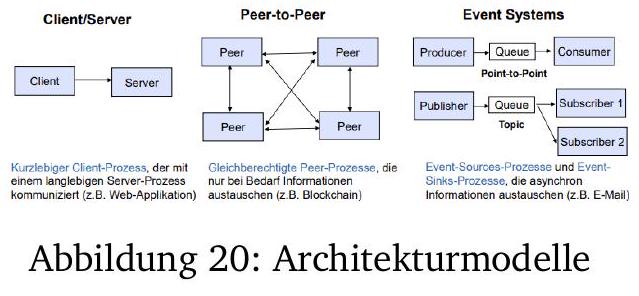
\includegraphics[max width=\textwidth, center]{2024_12_29_0d1d7b5551ea1b4b41bdg-18}

\subsection*{11.5 Gängige Technologien (Middleware) f. Informationssysteme und Internet-basierte Systeme}
Für die Entwicklung verteilter Systeme stehen verschiedene MiddlewareTechnologien zur Verfügung, die die Kommunikation und Integration von verteilten Komponenten erleichtern. Dazu gehören Messaging-Broker wie Apache

Kafka, Middleware-Frameworks wie CORBA (Common Object Request Broker Architecture) und RESTful Web Services.


\end{document}